\documentclass[12pt, titlepage]{article}
\usepackage[shortlabels]{enumitem}
\usepackage{comment}
\usepackage{booktabs}
\usepackage{tabularx}
\usepackage{hyperref}
\usepackage{float}
\usepackage{soul}
\usepackage{changepage}
\usepackage{graphicx}
\setstcolor{red}
\hypersetup{
    colorlinks,
    citecolor=black,
    filecolor=black,
    linkcolor=black,
    urlcolor=blue
}
\usepackage[dvipsnames]{xcolor}
\usepackage[round]{natbib}

%% Comments

\usepackage{color}

\newif\ifcomments\commentstrue %displays comments
%\newif\ifcomments\commentsfalse %so that comments do not display

\ifcomments
\newcommand{\authornote}[3]{\textcolor{#1}{[#3 ---#2]}}
\newcommand{\todo}[1]{\textcolor{red}{[TODO: #1]}}
\else
\newcommand{\authornote}[3]{}
\newcommand{\todo}[1]{}
\fi

\newcommand{\wss}[1]{\authornote{blue}{SS}{#1}} 
\newcommand{\plt}[1]{\authornote{magenta}{TPLT}{#1}} %For explanation of the template
\newcommand{\an}[1]{\authornote{cyan}{Author}{#1}}

%% Common Parts

\newcommand{\progname}{ProgName} % PUT YOUR PROGRAM NAME HERE
\newcommand{\authname}{Team \#, Team Name
\\ Student 1 name
\\ Student 2 name
\\ Student 3 name
\\ Student 4 name} % AUTHOR NAMES                  

\usepackage{hyperref}
    \hypersetup{colorlinks=true, linkcolor=blue, citecolor=blue, filecolor=blue,
                urlcolor=blue, unicode=false}
    \urlstyle{same}
                                


\setcitestyle{numbers}

\title{SE 4G06: Software Requirements Specification\\\textit{Measuring Microstructure Changes During Thermal Treatment }}

\author{\authname}

\date{}

\begin{document}

\maketitle

\pagenumbering{roman}
\tableofcontents
\listoftables
\listoffigures

\begin{table}[H]
\caption{\bf Revision History}
\begin{tabularx}{\textwidth}{p{2.5cm}p{2.5cm}X}
\toprule {\bf Date} & {\bf Developer} & {\bf Notes/Changes}\\
\midrule
Sept 25, 2022 & Edwin Do & Revision 0 - Initial commit\\
Oct 5, 2022 & Edwin Do & Adopt Volere template + Add content \\
Oct 5, 2022 & Timothy Chen & Added to Non-Functional Requirements\\
Oct 5, 2022 & Abdul Nour Seddiki & Added to Relevant Facts and Assumptions\\
Oct 5, 2022 & Abdul Nour Seddiki & Added to Waiting Room\\
Oct 5, 2022 & Timothy Chen & Added to Reflection\\
Oct 5, 2022 & Joseph Braun & Add functional Requirements \\ 
Oct 5, 2022 & Abdul Nour Seddiki & Added to Reflections\\
Oct 5, 2022 & Edwin Do & Add reflection + small fixes \\
Oct 6, 2022 & Edwin Do & Add missing tasks, ideas for solutions, and open issues \\
Oct 31, 2022 & Edwin Do & Update with the use of Visual Studio\\
Mar 8, 2023 & Abdul Nour Seddiki & Added two functional requirements\\
Apr 1, 2023 & Edwin Do & Added definitions for resistivity and conductivity\\
Apr 1, 2023 & Tyler Magarelli & Outlined variation from the template document \\
Apr 1, 2023 & Abdul Nour Seddiki & Added dangling section descriptions and fix spelling errors\\
Apr 1, 2023 & Joseph Braun & Added to Facts and updated Context Diagram\\
Apr 1, 2023 & Tyler Magarelli & Added Traceability Matrices\\
Apr 1, 2023 & Edwin Do & Revised requirements and use cases\\
\bottomrule
\end{tabularx}
\end{table}

\newpage

\pagenumbering{arabic}

\noindent This document describes the software requirements for the capstone project of measuring microstructure changes of samples during thermal treatment. The template for the Software Requirements Specification (SRS) is a subset of the Volere template. The section regarding likely changes was renamed to 'Waiting Room' and the team removed the section for unlikely changes. The 'Project Drivers' section encompasses the Introduction, General and Specific System description sections from the template. 

\section{Project Drivers}

This section will introduce the purpose of the project and the stakeholders, along with the requirement constraints and facts and terminology in order to set the scene about the project's main drivers.

\subsection{The Purpose of the Project}
The purpose of this project is to assist the Department of Materials Engineering in measuring the changes to a material's microstructure during thermal treatment. 
By doing so, the resistivity of the sample can be measured at different thermal levels. The goal is to be able to collect the data at the necessary sampling rate and 
incorporate the use of Windows GUI. 

\subsection{The Stakeholders}
The stakeholders will be introduced in this section, they include the developers, clients, and customers.

\subsubsection{Developers}
The Developers will be responsible for the design, development, and documentation throughout. They will be utilizing the existing lab equipment and computer for the duration of this project.
Developers will also use the feedback from the client to deliver the final product. 

\subsubsection{The Client}
The Client for this project is the Department of Materials Engineering and the Computing and Software Department at McMaster University. More specifically, Dr. Zurob, Dr. Smith, and the TAs of 4G06 will be the ones to evaluate, review and provide feedback on the project throughout the development process.

\subsubsection{The Customers}
The Customers for this project are anyone who will be conducting research or require data that measures the microstructural changes of materials under thermal treatment.   

\subsubsection{Other Stakeholders}
This project has no other stakeholders.

\subsection{Mandated Constraints}
This section outlines the general constraints of this project and categorizes them on a solution, software, environment, schedule, and budget constraints bases.

\subsubsection{Solution Constraints}

Description: The GUI will run on Windows operating systems\\ 
Rationale: The application is a Desktop application. The lab computer that has the capability to connect to other required lab equipment currently runs on Windows.\\
Fit Criterion: Users can successfully install and open the application on a supported Windows operating system. \\

\noindent Description: The sampling rate of the equipment to the GUI will be at least 100 times per second\\ 
Rationale: According to Dr. Zurob, this is the minimum sampling rate needed to see any meaningful data\\
Fit Criterion: The equipment samples the data at 100 times per second and the GUI accurately reflects the measurements  \\

\subsubsection{Off-the-shelf Software}
%No off-the-shelf software is required for this project. 
The application will use Visual Studio to create a WPF (Windows Presentation Foundation) application that will ensure compatibility with the lab Windows computer.

\subsubsection{Anticipated Workplace Environment}
The software and equipment will be designed for the expected environment of a lab. The reason is that the lab equipment and computer are needed for the software to run successfully and
should not be easily accessible outside of campus. 

\subsubsection{Schedule Constraints}
% Add other deadlines
The deadline for the final product is March 27, 2023. There will be other milestones during the development process that must be accomplished throughout. 
This will be outlined in our GitHub milestones.


\subsubsection{Budget Constraints}
% Double check this
At this point, there is an estimated budget of \$1000. This may change as the team determines what additional equipment is needed to work with the lab equipment.

\subsection{Naming Conventions and Terminology}

\begin{itemize}
    \item \textbf{C\#}: Scripting language used to create and control dynamic content.
    \item \textbf{Visual Studio}: Development IDE used to create a variety of applications
    \item \textbf{WPF}: Windows Presentation Foundation - Library used to create Windows Applications.
    \item \textbf{Windows}: A popular operating system used by many users.
    \item \textbf{GUI}: Graphical User Interface - A digital interface which allows the user to interact with electronic devices through graphical icons.
    \item \textbf{Product/Software/Application}: Refers to the final deliverable of this capstone project.
    \item \textbf{User}: The person who will be interacting/ using the application.
    \item \textbf{Resistivity}: A measure of the resisting power of specified material to the flow of an electric current.
    \item \textbf{Conductivity}: The ability to move heat or electricity from one place to another.
    \item \textbf{Data Acquisition Rate}: The internal clock timing of the instruments used in calculating measurements, the range is between MIN\_SAMPLE\_RATE and MAX\_SAMPLE\_RATE.
\end{itemize}

\subsection{Relevant Facts and Assumptions}
Facts, assumptions, and user characteristics that are relevant to the scope of this project are shown in this section.

\subsubsection{Facts}
The lab computer is using the Windows XP operating system which is questionably upgradeable and it is worth mentioning that Windows XP is currently unsupported. The equipment for power supply and measurement tools is outdated and requires special connection media, both physical connections and drivers, to communicate with the computer. There exists an application with a similar purpose and function to our project’s on the computer, which does not fulfill the goals of the user anymore, and the source code for that application is not provided.\\

\noindent Resistivity is the measure of the electrical resistance of a conductor of unit cross-sectional area and unit length. It is a characteristic property of each material and is useful for comparing materials on their ability to conduct electric currents. Conductivity is the measure of the ease at which an electric current can pass through a material. Conductivity is the inverse of resistivity. \\

\noindent Resistivity of sample material is calculated by the following equation. Where $\rho$ is the resistivity, R is the resistance, A is the cross-sectional area, and L is the length of the sample:
$ \rho = \frac{RA}{L} $
% Include a couple of sentences about the background and maybe an equation describing how the conductivity is calculated.

\subsubsection{Assumptions}
Statement: It is assumed that materials will have microstructural changes when they undergo heat treatment. 
Effect: In case this assumption is false, our product will display no output. \\

\noindent Statement: Another assumption is that these microstructural changes will result in changes in the resistivity of the materials treated. 
Effect: If this assumption is false, the product will be rendered unsuitable for the task as its main function is to measure changes in resistivity.\\

\noindent Statement: According to the project timeline, it is assumed that a proof of concept will be ready by November 14th, a first functional design will be ready by February 6th, and a final revision will be demoed by March 27th.
Effect: These dates are made to observe the progress of the project. In case the final demo is not met, the project will have been incomplete, since that will be the end-of-term for the developers.
% Include a couple of sentences about any assumptions that we have

\subsubsection{User Characteristics}
An assumption made about this project is that the users will have the necessary knowledge to safely operate the necessary lab equipment. This is required to collect the data and display it on the GUI. 
The user is also assumed to have a general working knowledge of how to install and open a Windows application, as well as the use of a mouse and keyboard input. Another assumption is that the user is literate in English.

\section{Functional Requirements}
The functional requirements section puts the functional needs of the stakeholders in context, shows possible use cases, and finally lists the functional requirements themselves.

\subsection{The Scope of the Work and the Product}

The hardware for this project is provided by the Department of Materials Engineering through the project supervisor, Dr. Zurob. A Windows computer, current source, and nanovoltmeter have already been included. A fourth hardware device, for measuring the temperature of the sample material, will also be provided or else a new device shall be purchased for this purpose. The product will be a Windows-based GUI application that can set the data acquisition rate, connect to the hardware devices, acquire the output data, and calculate the conductivity of the sample material in real time. The application should also be able to be accessed remotely to check on the progress of ongoing experiments. \\

\subsubsection{The Context of the Work}
% Electron - JS, HTML , CSS
% CI/CD - Build
% Devs may require the use of other libraries to speed up the dev process
\begin{figure}[H]
\centerline{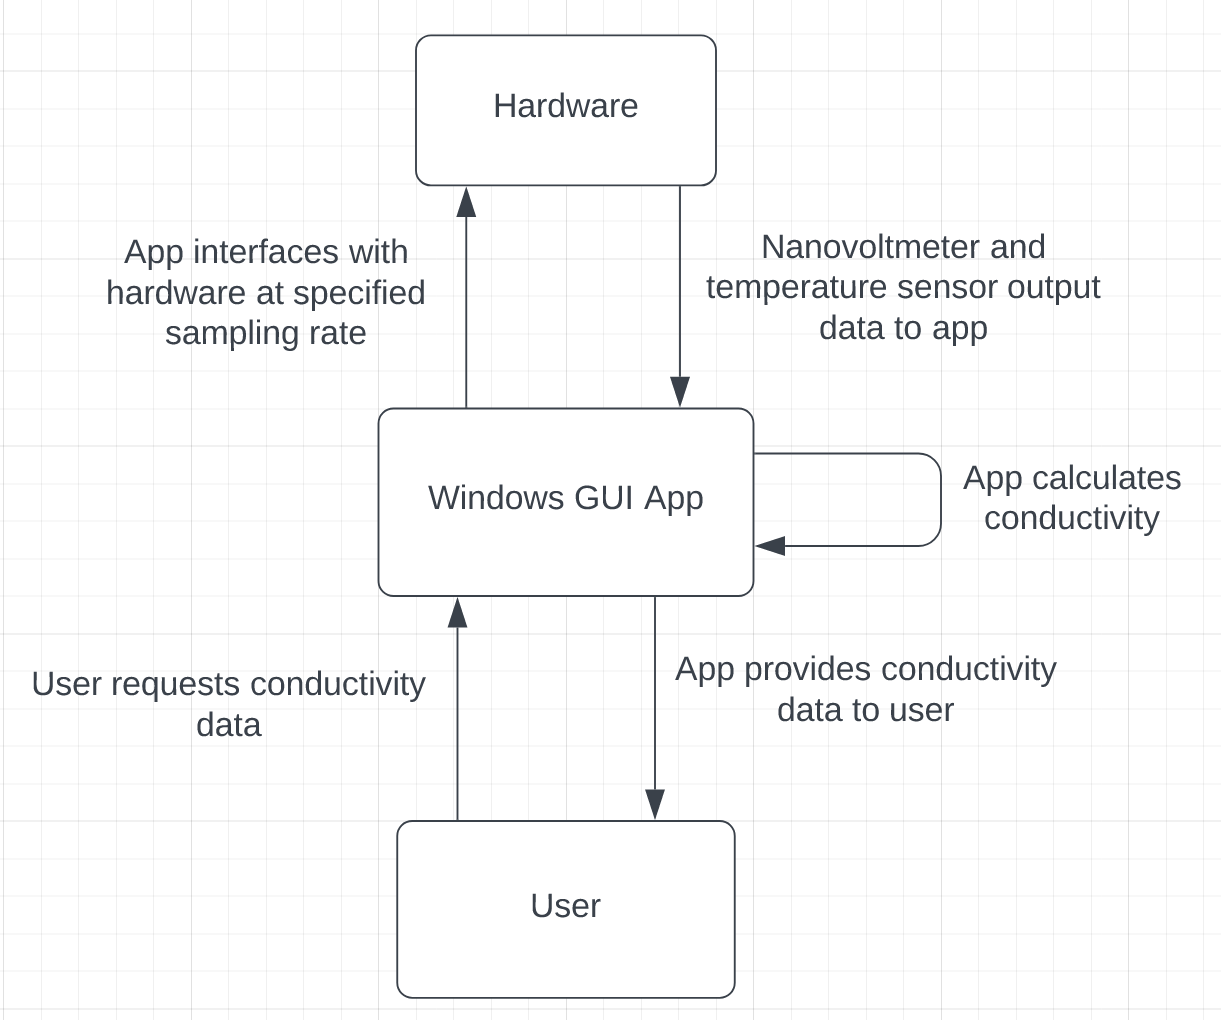
\includegraphics[scale=0.9]{ContextDiagram.PDF}}
\caption{Basic context diagram (subject to change as the project progresses)}
\label{fig}
\end{figure}

\subsubsection{Work Partitioning}

\begin{table}[H]
	\centering
	\caption{Work Partitioning}
	\label{my-label}
	\begin{tabular}{|c|c|c|c|}
		\hline
		\textbf{Event \#} & \textbf{Event Name} & \textbf{Input} & \textbf{Output}     \\ \hline
		1 & \begin{tabular}{@{}c@{}}User requests\\resistivity data\end{tabular} & 
            \begin{tabular}{@{}c@{}}Data\\request\end{tabular} & 
            \begin{tabular}{@{}c@{}}Resistivity\\data\end{tabular} \\ \hline
		2 & \begin{tabular}{@{}c@{}}App connects\\to hardware\end{tabular} & 
            \begin{tabular}{@{}c@{}}Data\\sampling rate\end{tabular} & 
            \begin{tabular}{@{}c@{}}Voltage and\\temperature data\end{tabular} \\ \hline
		3 & \begin{tabular}{@{}c@{}}App calculates\\resistivity\end{tabular} & 
            \begin{tabular}{@{}c@{}}Voltage and\\temperature data\end{tabular} & 
            \begin{tabular}{@{}c@{}}Sample\\resistivity\end{tabular}  \\ \hline
	\end{tabular}
\end{table}

\begin{table}[H]
	\centering
	\caption{Work Partitioning - Description}
	\label{my-label}
	\begin{tabular}{|c|c|}
		\hline
		\textbf{Event \#} & \textbf{Description}											\\ \hline
		1 & \begin{tabular}{@{}c@{}}User opens app and requests resistivity data\\for the current sample connected to hardware\end{tabular}	\\ \hline
		2 & \begin{tabular}{@{}c@{}}App interfaces with hardware, sets sampling rate,\\and records data from hardware\end{tabular}	\\ \hline
		3 & \begin{tabular}{@{}c@{}}App uses data received from hardware to calculate\\resistivity of sample\end{tabular}  \\ \hline
	\end{tabular}
\end{table}


\subsubsection{Individual Product Use Cases}

\begin{enumerate}[{UC-}1:]
    
%--Use Case Template
\item Install and use the application in the lab to measure resistivity changes in sample material \label{UC1}\\
    \textbf{Related Requirements:} \ref{FR1}, \ref{FR2}, \ref{FR3}, \ref{FR4}, \ref{FR8}\\ %Cross reference with requirements below
    \textbf{Initiating Actor:} The User\\
    \textbf{Actor's Goal:} Record resistivity changes in sample material during thermal treatment\\
    \textbf{Participating Actors:} User, Application, Hardware\\
    \textbf{Pre-conditions:} User in lab; sample material connected to hardware\\
    \textbf{Flow of events for main success:}\\
    $\rightarrow$ 1. The user installs and opens the application\\
    $\rightarrow$ 2. The user starts the experiment\\
    $\rightarrow$ 3. The user requests resistivity data from the application\\
    $\rightarrow$ 4. The application interfaces with hardware\\
    $\leftarrow$ 5. Hardware outputs voltage and temperature data to the application\\
    $\leftarrow$ 6. The application calculates and outputs resistivity data to the user\\

\item Control the lab devices remotely while an experiment that monitors resistivity changes is running \label{UC2}\\
    \textbf{Related Requirements:} FR1, FR2, FR3, FR4, FR5\\ %Cross reference with requirements below
    \textbf{Initiating Actor:} The User\\
    \textbf{Actor's Goal:} Monitor resistivity changes in sample material remotely during thermal treatment\\
    \textbf{Participating Actors:} User, Application, Hardware\\
    \textbf{Pre-conditions:} The user remotely connected to the application; sample material connected to hardware\\
    \textbf{Flow of events for main success:}\\
    $\rightarrow$ 1. The user requests to turn on the current output\\
    $\leftarrow$ 2. The request is relayed over a network to the application\\
    $\leftarrow$ 3. The application interfaces with hardware\\
    $\rightarrow$ 4. The current output is turned on\\
    $\leftarrow$ 5. The application checks the status of the current output\\
    $\leftarrow$ 6. The application sends confirmation back to the user remotely

\item Use the application to view a visual representation of the data and export it to a file that can be saved in other file locations \label{UC3}\\
    \textbf{Related Requirements:} FR6, FR7\\ %Cross reference with requirements below
    \textbf{Initiating Actor:} The User\\
    \textbf{Actor's Goal:} See a visual output of captured data and save it\\
    \textbf{Participating Actors:} User, Application\\
    \textbf{Pre-conditions:} User is successfully running an experiment that is capturing data
    \textbf{Flow of events for main success:}\\
    $\rightarrow$ 1. The user stops capture\\
    $\rightarrow$ 2. The user uses the graphical display and its tools to analyze data visually\\
    $\rightarrow$ 3. The user requests the application to output the graphical data\\
    $\leftarrow$ 4. A file containing an image of the graphical display is outputted to the computer\\
    $\leftarrow$ 5. The user requests the application to output the captured data\\
    $\leftarrow$ 6. A file containing the data of the captured data is outputted to the computer
    
\color{black}
\end{enumerate}

\subsection{Functional Requirements}
% List functional requirements here
\begin{enumerate}[{FR}1.] 
    \item \label{FR1}
    The app shall monitor the resistivity of the sample material in real time. 
    \item \label{FR2}
    The app shall change the data sampling rate as required.
    % \item \label{FR3}
    % The app shall automate the process of identifying slope changes and correlating these to phase changes in the sample. 
    \item \label{FR3}
    The app shall have remote access and control.
    \item \label{FR4}
    The app shall display measurements and calculations in a graph.
    \item \label{FR5}
    The app shall have a file output system.
    \item \label{FR6}
    The app shall be able to be installed on a Windows computer. \\
	
\end{enumerate}

\section{Non-functional Requirements}
This section puts the requirements that are not necessarily essential to the function of the product into perspective. Requirements such as the look, usability, performance, security, and legal requirements are specified below.

\subsection{Look and Feel Requirements}
\begin{adjustwidth}{2.2em}{0pt}
\begin{enumerate}[{NFR-L}1.]
   \item The product shall feel simple to use.\\ \label{NFR-L1}
   Fit Criterion: Survey should reflect 90 percent of users should feel like the product is uncomplicated to use.
   \item The product shall be in English only.\\\label{NFR-L2}
   Fit Criterion: The language used throughout the product will be in English.
\end{enumerate}
\end{adjustwidth}
 

\subsection{Usability and Humanity Requirements}
\begin{adjustwidth}{2.2em}{0pt}
\begin{enumerate}[{NFR-U}1.]
  \item Users with no prior experience with the product should be able to use it.\\ \label{NFR-U1}
  Fit Criterion: New user will be able to complete each task successfully within 1 minute. 
  \item Product shall have a straightforward interface allowing for quick modifications to parameters with ease.\\ \label{NFR-U2}
  Fit Criterion: The time between the user interacting with the application and modifying a parameter to change it in the interface should be no longer than INTERACT\_TIME.
  \item Product shall help the user accurately make modifications and avoid mistakes.\\ \label{NFR-U3}
  Fit Criterion: The total number of mistakes made by the user should be no more than MAX\_MISTAKE when completing a set of tasks. 
  \item Users should be able to learn the use of the product over time.\\ \label{NFR-U4}
  Fit Criterion: User will be able to complete a set of tasks faster the next day for the second time compared to the first time.
  \item The product shall conceal detailed structures and calculations from the user.\\ \label{NFR-U5}
  Fit Criterion: The product will not show any calculations used for producing output based on the user's parameters.
  \item The capacity of the product shall not be large.\\ \label{NFR-U6}
  Fit Criterion: The product will be no more than MAX\_SIZE.
\end{enumerate}
\end{adjustwidth}

\subsection{Performance Requirements}
\begin{adjustwidth}{2.2em}{0pt}
\begin{enumerate}[{NFR-P}1.]
  \item The product shall be able to read at MIN\_SAMPLE\_RATE\\ \label{NFR-P1}
  Fit Criterion: The rate of reading will be measured and the rate determined by the measurement shall be no less than MIN\_SAMPLE\_RATE. 
  \item Changes to the parameters will be reflected in the product within TIME\_ACCEPTED of the user's input.\\ \label{NFR-P2}
  Fit Criterion: The product will reflect changes given by the user within TIME\_ACCEPTED. 
  \item The product shall read measurements and calculations shall be accurate to ACCEPTED\_SIGFIG.\\ \label{NFR-P3}
  Fit Criterion: The measurements and calculations will be verified to ACCEPTED\_SIGFIG.
  \item When the user is using the product, it shall be up and running for at least MIN\_UPTIME.\\ \label{NFR-P4}
  Fit Criterion: The product will be up and running during the interactions with the user and for at least MIN\_UPTIME after.
\end{enumerate}
\end{adjustwidth}

\subsection{Operational and Environmental Requirements}
\begin{adjustwidth}{2.2em}{0pt}
\begin{enumerate}[{NFR-O}1.]
  \item Product should accept inputs from keyboard and mouse.\\ \label{NFR-O1}
  Fit Criterion: The keyboard and mouse connected to the computer will be able to interact with the product.
  \item Product shall be able to be installed by a user with no prior experience with the product on a Windows Computer.\\ \label{NFR-O2}
  Fit Criterion: User with no prior experience of installing the application should be able to install the application with the optional assistance of an user guide.
  % \item Releases occur at least once every 6 months.\\
  % Fit Criterion: The team will make a release with minor bug fixes and new features if needed at least once every 6 months.
\end{enumerate}
\end{adjustwidth}

\subsection{Maintainability and Support Requirements}
\begin{adjustwidth}{2.2em}{0pt}
\begin{enumerate}[{NFR-M}1.] 
  % \item Major bugs or issues brought up by the user shall be handled within 72 hours of receiving it.\\
  % Fit Criterion: Bugs or issues will be handled by developers within 48 hrs and will be escalated after so it can be resolved by 72 hour mark.
  \item Product shall work on Windows 10/11 operating systems.\\ \label{NFR-M1}
  Fit Criterion: The product will be installed on the operating system and have its functions verified.
  \item Product shall be expected to work on the computers in the lab.\\ \label{NFR-M2}
  Fit Criterion: The product will be installed and used as expected on the lab's computer.
\end{enumerate} 
\end{adjustwidth}

\subsection{Security Requirements}
\begin{adjustwidth}{2.0em}{0pt}
\begin{enumerate}[{NFR-S}1.]
  \item The product shall prevent modifications or injections of measurements.\\ \label{NFR-S1}
  Fit Criterion: The product will only allow users to read measurements and deny any attempts to change them.
  \item Only authorized users are allowed to modify concealed calculations, settings, and/or parameters.\\ \label{NFR-S2}
  Fit Criterion: Users who have clearance will have access to modify certain calculations and parameters.
\end{enumerate}
\end{adjustwidth}

\subsection{Cultural Requirements}
\begin{adjustwidth}{2.2em}{0pt}
\begin{enumerate}[{NFR-C}1.]
    \item The product must not include any graphics or wording that may be considered offensive or inappropriate to the user.\\ \label{NFR-C1}
    Fit Criterion: To measure this, a usability survey will be conducted. User indicating they agree or strongly agree graphics and wording are not offensive or inappropriate will be considered successful.
\end{enumerate}
\end{adjustwidth}

\subsection{Legal Requirements}
\begin{adjustwidth}{2.7em}{0pt}
\begin{enumerate}[{NFR-LR}1.]
    N/A
\end{enumerate}
\end{adjustwidth}

\subsection{Health and Safety Requirements}
\begin{adjustwidth}{2.2em}{0pt}
\begin{enumerate}[{NFR-H}1.]
  % Add item about lab safety  
  % \item ADD TEXT HERE
  \item Colours and graphics used in the application should take into account users who may be prone to seizures. \\ \label{NFR-H1}
    Fit Criterion: There should be no animations that simulate flashing/ flickering (i.e change of brightness or colour at a rapid rate). There should also be no static optical illusions that may simulate any flashing/ flickering.
    \item Colours should not be too bright, causing potential harm to users' eyes. \\ \label{NFR-H2}
    Fit Criterion: Colours of the GUI should be checked to ensure it does not simulate extra light. Example: colours that include the words 'bright,' 'flashy' or 'neon'.
\end{enumerate}
\end{adjustwidth}

\subsection{Installability Requirements}
\begin{adjustwidth}{2.0em}{0pt}
\begin{enumerate}[{NFR-I}1.]
  \item Product requires a Windows computer with the necessary ports to connect to the lab equipment. \\ \label{NFR-I1}
    Fit Criterion: Copy over the zipped file with the executable within to the new computer. Unzip the folder and open the application to see if the readings from the lab equipment are reflected correctly.
\end{enumerate}
\end{adjustwidth}

\section{Project Issues}
This section will go into detail on the lists of next items to address, off-the-shelf solutions, potential problems, risks, costs, ideas, and waiting room items.

\subsection{Open Issues}
% What are some issues we have right now
\begin{itemize}
  \item Determine maintainability and stability of the Windows XP operating system
  \item Identify the best-suited method for communication between lab equipment and the application
  \item Identify the appropriate hardware and software development to ensure the best sampling rates
  \item Investigate the necessary drivers, if any, on the lab computer for it to work with the lab equipment
\end{itemize}

\subsection{Off-the-Shelf Solutions}
The application will use Visual Studio to create a WPF (Windows Presentation Foundation) application that will ensure compatibility with the lab Windows computer.

% The application will use Electron, a JavaScript framework that allows developers to create cross-platform compatible desktop applications. 
% Since the use cases of this project are more specialized, there are not many existing solutions available on the market.

\subsubsection{Ready Made Components}

The application will use many of the existing IDE extensions in Visual Studio to further support communication with any equipment in the lab.
% The application will use existing libraries in Electron to further support the communication with any equipment in the lab.

\subsection{New Problems}
 A potential problem from our product that may arise is the user's ability to learn the software.
  \subsubsection{Potential User Problems}
This product introduces a new learning curve for the user to use the application. 
To minimize this problem, the product will be implemented with a quick start guide and developers will design a user-friendly interface.


\subsection{Tasks}
% What do we need to do?
% Communicate lab equipment output to some kind of communication channel (serial port, sockets, named pipes)
% Read data from the communication channel
% Create a GUI that can be installed and run on Windows 7
\begin{itemize}
  \item Find and create a method of communication between the lab equipment and the application (i.e. serial ports, named pipes, inter-process communication)
  \item Accurately read the data output in real-time from the application
  \item Create a GUI that can be installed and successfully run on a Windows 10 operating system
\end{itemize}

\subsection{Migration to the New Product}
N/A

\subsection{Risks}
A risk to this project is that the current lab computer has special ports to communicate with the necessary hardware equipment. Although creating a WPF application should help with compatibility on Windows computers,
there is a risk to whether the necessary drivers are available and if the communication will still work after upgrading to Windows 10. \\
% A risk to this project is that the current lab computer uses Windows 7 as its operating system. Although Electron has compatiblity with Windows 7, there appears to be a few issues in the past on GitHub. 
% In the case that it does not work, the operating system will have to be upgraded to Windows 10 and the compatibility with the lab equipment is uncertain. Additionally, McMaster University had notified the 
% Department of Materials Engineering that Windows 7 is no longer supported but since the lab computer does not require any network connections, it has remained running Windows 7. This poses a future risk of 
% the operating system being forcefully upgraded.\\

\noindent Another risk is that the lab equipment does not offer the necessary sampling or is not compatible with the lab computer. 

\subsection{Costs}
The largest estimated cost of this project is time. It will require both the developers and the client's time to work on and evaluate the project throughout.
Additional expenses may be added if additional or new lab equipment is required. 

\subsection{User Documentation and Training}
A main README file will be created and documented for information such as installation, system requirements, and available features. 
An additional safety document will also be created for users, before using any of the lab equipment. 

\subsection{Waiting Room}
\begin{itemize}
    \item Requiring the highest possible rate of output.
    \item Requiring the software to work on the latest (supported) version of Windows.
    \item The option of using the application remotely.
    \item The option of using the application on different platforms, operating systems, devices, and with different input and measurement tools.
    \item Ability of the system to be a real-time system where it is used concurrently with the heat treatment process of materials, connected to the heat treatment systems and controlling them, measuring changes in real-time, and making decisions on the fly.
    \item Incorporation of machine learning and artificial intelligence in order to analyze data within processes and make adjustments to the treatment for customized optimal results.
    \item Addition of other methods of measurement of microstructural change; like adding high-speed electronic microscopes with slow-motion capture for manual or automated analysis of the physical outputs.
\end{itemize}

\subsection{Ideas for Solutions}
% Electron
% Serial ports and communication
% Use electron libraries
\begin{itemize}
  \item Use Electron to create Desktop Application
  \item Use Visual Studio to create UWP/WPF (Windows Presentation Foundation) Application
  \item Write the data from the lab equipment to a serial port for communication with the application
  \item Utilize electron libraries to support communication on a serial port
  \item Utilize inter-process communication for communication between the lab equipment and application
\end{itemize}


\bibliographystyle{plainnat}

%\bibliography{SRS}

\section{Traceability Matrix}
In this section, an overview of the relationships between use cases and functional requirements, and other relationships between functional and non-functional requirements are provided. This allows for easy bi-directional navigation and ensures all requirements and use cases are accounted for.

\begin{table}[h]
\centering
\begin{tabular}{|c|c|c|c|c|c|c|c|}
\hline        
	 & \ref{FR1} & \ref{FR2}& \ref{FR3} & \ref{FR4} & \ref{FR5}& \ref{FR6} & \ref{FR7} &
\hline
\ref{UC1}     & X & X & X & & & & X\\ \hline
\ref{UC2}     & X & X & X & X & & & \\ \hline
\ref{UC3}     &   &  &  &  & X & X &\\ \hline
\hline
\end{tabular}
\caption{Traceability Matrix Showing the Connections Between Use Cases and Functional Requirements}
\label{Table:trace}
\end{table}

\begin{table}[h!]
\centering
\begin{tabular}{|c|c|c|c|c|c|c|}
\hline        
	 & \ref{FR1} & \ref{FR2}& \ref{FR3} & \ref{FR4} & \ref{FR5}& \ref{FR6} &
\hline
\ref{NFR-L1}     &  &  &  & X & X & \\ \hline
\ref{NFR-L2}     &  &  &  &  &  & \\ \hline
\ref{NFR-U1}     &  &  &  &  &  & \\ \hline
\ref{NFR-U2}     &  &  & X &  &  & \\ \hline
\ref{NFR-U3}     &  & X &  & X & X & \\ \hline
\ref{NFR-U4}     &  &  &  &  &  &  \\ \hline
\ref{NFR-U5}     &  &  &  &  &  & \\ \hline
\ref{NFR-U6}     &  &  &  &  &  & \\ \hline
\ref{NFR-P1}     &  & X &  &  &  & \\ \hline
\ref{NFR-P2}     & X &  & X & X &  & \\ \hline
\ref{NFR-P3}     & X &  &  & X & X & \\ \hline
\ref{NFR-P4}     & X &  &  &  &  & \\ \hline
\ref{NFR-O1}     &  &  &  &  &  & \\ \hline
\ref{NFR-O2}     &  &  &  &  &  & \\ \hline
\ref{NFR-M1}     &  &  &  &  &  & \\ \hline
\ref{NFR-M2}     &  &  &  &  &  & \\ \hline
\ref{NFR-S1}     & X &  &  &  &  & \\ \hline
\ref{NFR-S2}     &  &  &  &  &  & \\ \hline
\ref{NFR-C1}     &  &  &  & X & X & \\ \hline
\ref{NFR-H1}     &  &  &  & X & X & \\ \hline
\ref{NFR-H2}     &  &  &  & X & X & \\ \hline
\ref{NFR-I1}     &  &  &  &  &  & X\\ \hline
\hline
\end{tabular}
\caption{Traceability Matrix Showing the Connections Between Functional and Non-Functional Requirements}
\label{Table:trace}
\end{table}

\clearpage
\newpage
\section{Appendix}

This section contains a table making reference to symbolic parameters used throughout the document.

\subsection{Symbolic Parameters}

% \begin{itemize}
%     \color{red}
%     \item \hyperref[sec:sampling]{SAMPLING\_RATE\_PER\_SECOND = 100}
% \end{itemize}

\begin{tabular}{l l} 
  \toprule		
  \textbf{symbol} & \textbf{description}\\
  \midrule 
  TARGET\_TIME & 60 seconds \\
  INTERACT\_TIME & 5 seconds \\
  MAX\_MISTAKE & 2 \\
  MAX\_SIZE & 8GB \\ 
  MIN\_UPTIME & 30 minutes \\ 
  MIN\_SAMPLE\_RATE & 60 samples per second\\
  MAX\_SAMPLE\_RATE & 600 samples per second\\
  TIME\_ACCEPTED & 1 second \\
  ACCEPTED\_SIGFIG & 3 decimals \\
  \bottomrule
\end{tabular}\\

\section{Phase In Plan / Development Plan}

\begin{table}[h!]
\centering
\begin{tabular}{|c|c|c|}
\hline        
	Priority & Functional Requirement & Planned Completion Date & 
\hline
1     & \ref{FR1} & November 10, 2022 &  \hline
2     & \ref{FR6} & November 15, 2022 &  \hline
3     & \ref{FR5} & November 24, 2022 &  \hline
5     & \ref{FR2} & December 12, 2022  & \hline
6     & \ref{FR4} & January 17, 2023 &  \hline
7     & \ref{FR3} & February 3, 2023 &  \hline
     
\hline
\end{tabular}
\caption{Development Plan chart that highlights priorities of development and planned completion dates.}
\label{Table:table}
\end{table}

\section{Reflections}

\noindent Q1: What knowledge and skills will the team collectively need to acquire to successfully complete this capstone project? \\
% Examples of possible knowledge to acquire include domain-specific knowledge from the domain of your application, 
% software engineering knowledge, mechatronics knowledge or computer science knowledge. 
% Skills may be related to technology, writing, presentation, team management, etc. You should look to identify at least one item for each team member.
\noindent Q2: For each of the knowledge areas and skills identified in the previous question, what are at least two approaches to acquiring the knowledge or mastering the skill? 
From the identified approaches, which will each team member pursue, and why did they make this choice?\\

\noindent Responses\\


Timothy - We need to acquire the knowledge and skills on developing a Window application using the Electron as the framework. One of the main requirements
from the supervisor is that it has to work on Windows operating systems. In my experience through Co-op and school work, I have 
yet to interact with Windows applications. This knowledge will hope us meet the requirements set by the supervisor as well 
as learn a new technical skill. 

There are a few approaches to acquiring this knowledge. The first way would be to look for blogs from other developers and learn from their
examples. The second way would be to watch and read tutorials online. The third way would be to read the documentation and conduct research. Lastly, 
we could also learn by trial and error. The approach I will be taking will be watching and reading tutorials online as they will be able to explain 
concepts in a simpler form with visual aids. This will help me gain knowledge in this concept and 
make it a skill I can gain from this project.\\

Abdul - The team needs to learn about programming in relation to signal inputs and outputs. Potentially signal processing knowledge would be involved. Another aspect we will need to learn about is simple circuit design specifically for testing metallic specimens, which involves dealing with current sources and nanovoltmeters.

Online resources are a very good candidate for these skills. Mostly happening through continuous research along with trial and error. Some material science-specific questions could be raised to Dr. Zurob.\\

Joseph - One of the main components of the project will be to interface the Windows application with the hardware. Since none of the team members has worked with this particular hardware setup before, this will be new knowledge we are required to learn.  

There are two main ways I can think of to acquire this knowledge. The first way would be to use the old Windows application which is currently installed on the lab computer. This application could be reverse-engineered to determine how the software interfaced with the hardware, and then this method could be copied for our own application. A second way would be to study the data sheets and/or user manuals of the hardware in order to learn how the hardware is designed to interface with software. The approach I will be taking is the latter. I may find out through this approach that there is more than one possible method, in which case we could choose the one most suitable for our needs rather than be limited to one method.\\ 

Edwin - The group needs to collectively learn Electron, a JavaScript framework that the team is planning on utilizing to develop the desktop application. In addition, the group will also need to collectively learn different methods of how to enable communication between the lab equipment and the application. An example of this may be inter-process communication.

Two approaches to learning Electron as a new framework would be to create a prototype and follow online tutorials. For myself, I will approach learning Electron by creating quick prototypes that accomplish a task we need. This may be supplemented by reading available documentation.

Learning the different methods that allow hardware and software to communicate will require research and tutorials. By researching we can learn the strengths and weaknesses to determine which method is best suited for our project. Tutorials will help provide quick hands-on experience on how to get communication to work.

Tyler - The group needs to learn how to use a JavaScript framework to receive inputs from external hardware. 

This can be done through extensive research into the framework at hand and its built-in libraries and functionality. Starting with small partitioned tasks and increasing in size and difficulty slowly will help us to fully understand how to use it all.


\end{document}